% Created by tikzDevice version 0.12.6 on 2026-10-30 12:54:46
% !TEX encoding = UTF-8 Unicode
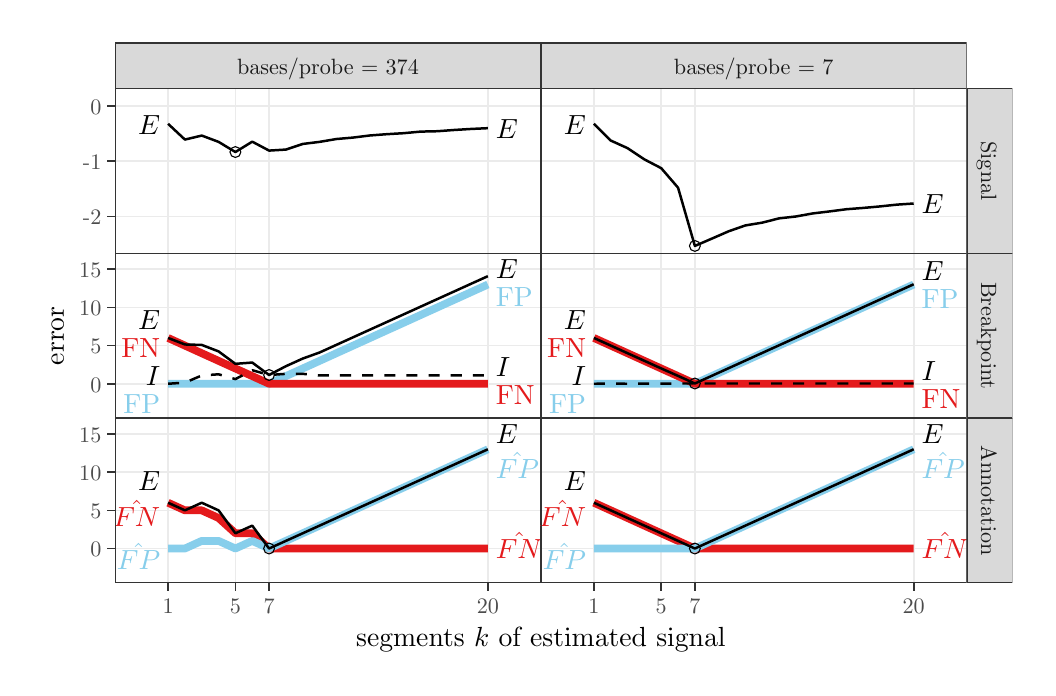
\begin{tikzpicture}[x=1pt,y=1pt]
\definecolor{fillColor}{RGB}{255,255,255}
\path[use as bounding box,fill=fillColor,fill opacity=0.00] (0,0) rectangle (361.35,231.26);
\begin{scope}
\path[clip] (  0.00,  0.00) rectangle (361.35,231.26);
\definecolor{drawColor}{RGB}{255,255,255}
\definecolor{fillColor}{RGB}{255,255,255}

\path[draw=drawColor,line width= 0.6pt,line join=round,line cap=round,fill=fillColor] (  0.00, -0.00) rectangle (361.35,231.26);
\end{scope}
\begin{scope}
\path[clip] ( 31.58,149.69) rectangle (185.45,209.23);
\definecolor{fillColor}{RGB}{255,255,255}

\path[fill=fillColor] ( 31.58,149.69) rectangle (185.45,209.23);
\definecolor{drawColor}{gray}{0.92}

\path[draw=drawColor,line width= 0.6pt,line join=round] ( 31.58,162.99) --
	(185.45,162.99);

\path[draw=drawColor,line width= 0.6pt,line join=round] ( 31.58,183.01) --
	(185.45,183.01);

\path[draw=drawColor,line width= 0.6pt,line join=round] ( 31.58,203.04) --
	(185.45,203.04);

\path[draw=drawColor,line width= 0.6pt,line join=round] ( 50.74,149.69) --
	( 50.74,209.23);

\path[draw=drawColor,line width= 0.6pt,line join=round] ( 75.06,149.69) --
	( 75.06,209.23);

\path[draw=drawColor,line width= 0.6pt,line join=round] ( 87.23,149.69) --
	( 87.23,209.23);

\path[draw=drawColor,line width= 0.6pt,line join=round] (166.29,149.69) --
	(166.29,209.23);
\definecolor{drawColor}{RGB}{0,0,0}

\path[draw=drawColor,line width= 0.9pt,line join=round] ( 50.74,196.51) --
	( 56.82,190.82) --
	( 62.90,192.27) --
	( 68.98,189.99) --
	( 75.06,186.32) --
	( 81.15,190.07) --
	( 87.23,186.84) --
	( 93.31,187.21) --
	( 99.39,189.24) --
	(105.47,189.99) --
	(111.55,191.02) --
	(117.64,191.55) --
	(123.72,192.31) --
	(129.80,192.77) --
	(135.88,193.13) --
	(141.96,193.70) --
	(148.04,193.84) --
	(154.13,194.29) --
	(160.21,194.66) --
	(166.29,194.94);

\path[draw=drawColor,line width= 0.4pt,line join=round,line cap=round] ( 75.06,186.32) circle (  1.96);
\end{scope}
\begin{scope}
\path[clip] ( 31.58,149.69) rectangle (185.45,209.23);
\definecolor{drawColor}{RGB}{0,0,0}

\node[text=drawColor,anchor=base east,inner sep=0pt, outer sep=0pt, scale=  1.00] at ( 47.89,192.74) {$E$};

\node[text=drawColor,anchor=base west,inner sep=0pt, outer sep=0pt, scale=  1.00] at (169.14,191.17) {$E$};
\definecolor{drawColor}{gray}{0.20}

\path[draw=drawColor,line width= 0.6pt,line join=round,line cap=round] ( 31.58,149.69) rectangle (185.45,209.23);
\end{scope}
\begin{scope}
\path[clip] ( 31.58, 90.15) rectangle (185.45,149.69);
\definecolor{fillColor}{RGB}{255,255,255}

\path[fill=fillColor] ( 31.58, 90.15) rectangle (185.45,149.69);
\definecolor{drawColor}{gray}{0.92}

\path[draw=drawColor,line width= 0.6pt,line join=round] ( 31.58,102.59) --
	(185.45,102.59);

\path[draw=drawColor,line width= 0.6pt,line join=round] ( 31.58,116.38) --
	(185.45,116.38);

\path[draw=drawColor,line width= 0.6pt,line join=round] ( 31.58,130.17) --
	(185.45,130.17);

\path[draw=drawColor,line width= 0.6pt,line join=round] ( 31.58,143.96) --
	(185.45,143.96);

\path[draw=drawColor,line width= 0.6pt,line join=round] ( 50.74, 90.15) --
	( 50.74,149.69);

\path[draw=drawColor,line width= 0.6pt,line join=round] ( 75.06, 90.15) --
	( 75.06,149.69);

\path[draw=drawColor,line width= 0.6pt,line join=round] ( 87.23, 90.15) --
	( 87.23,149.69);

\path[draw=drawColor,line width= 0.6pt,line join=round] (166.29, 90.15) --
	(166.29,149.69);
\definecolor{drawColor}{RGB}{135,206,235}

\path[draw=drawColor,line width= 2.8pt,line join=round] ( 50.74,102.59) --
	( 56.82,102.59) --
	( 62.90,102.59) --
	( 68.98,102.59) --
	( 75.06,102.59) --
	( 81.15,102.59) --
	( 87.23,102.59) --
	( 93.31,105.35) --
	( 99.39,108.10) --
	(105.47,110.86) --
	(111.55,113.62) --
	(117.64,116.38) --
	(123.72,119.14) --
	(129.80,121.90) --
	(135.88,124.65) --
	(141.96,127.41) --
	(148.04,130.17) --
	(154.13,132.93) --
	(160.21,135.69) --
	(166.29,138.45);
\definecolor{drawColor}{RGB}{228,26,28}

\path[draw=drawColor,line width= 2.8pt,line join=round] ( 50.74,119.14) --
	( 56.82,116.38) --
	( 62.90,113.62) --
	( 68.98,110.86) --
	( 75.06,108.10) --
	( 81.15,105.35) --
	( 87.23,102.59) --
	( 93.31,102.59) --
	( 99.39,102.59) --
	(105.47,102.59) --
	(111.55,102.59) --
	(117.64,102.59) --
	(123.72,102.59) --
	(129.80,102.59) --
	(135.88,102.59) --
	(141.96,102.59) --
	(148.04,102.59) --
	(154.13,102.59) --
	(160.21,102.59) --
	(166.29,102.59);
\definecolor{drawColor}{RGB}{0,0,0}

\path[draw=drawColor,line width= 0.9pt,dash pattern=on 4pt off 4pt ,line join=round] ( 50.74,102.59) --
	( 56.82,102.99) --
	( 62.90,105.58) --
	( 68.98,106.01) --
	( 75.06,104.27) --
	( 81.15,107.49) --
	( 87.23,105.75) --
	( 93.31,106.17) --
	( 99.39,106.17) --
	(105.47,105.60) --
	(111.55,105.60) --
	(117.64,105.60) --
	(123.72,105.60) --
	(129.80,105.60) --
	(135.88,105.60) --
	(141.96,105.60) --
	(148.04,105.60) --
	(154.13,105.60) --
	(160.21,105.60) --
	(166.29,105.60);

\path[draw=drawColor,line width= 0.9pt,line join=round] ( 50.74,119.14) --
	( 56.82,116.78) --
	( 62.90,116.62) --
	( 68.98,114.28) --
	( 75.06,109.79) --
	( 81.15,110.25) --
	( 87.23,105.75) --
	( 93.31,108.93) --
	( 99.39,111.69) --
	(105.47,113.88) --
	(111.55,116.64) --
	(117.64,119.40) --
	(123.72,122.16) --
	(129.80,124.91) --
	(135.88,127.67) --
	(141.96,130.43) --
	(148.04,133.19) --
	(154.13,135.95) --
	(160.21,138.71) --
	(166.29,141.46);

\path[draw=drawColor,line width= 0.4pt,line join=round,line cap=round] ( 87.23,105.75) circle (  1.96);
\end{scope}
\begin{scope}
\path[clip] ( 31.58, 90.15) rectangle (185.45,149.69);
\definecolor{drawColor}{RGB}{228,26,28}

\node[text=drawColor,anchor=base east,inner sep=0pt, outer sep=0pt, scale=  1.00] at ( 47.89,112.15) {FN};

\node[text=drawColor,anchor=base west,inner sep=0pt, outer sep=0pt, scale=  1.00] at (169.14, 95.27) {FN};
\definecolor{drawColor}{RGB}{0,0,0}

\node[text=drawColor,anchor=base east,inner sep=0pt, outer sep=0pt, scale=  1.00] at ( 47.89,102.04) {$I$};

\node[text=drawColor,anchor=base west,inner sep=0pt, outer sep=0pt, scale=  1.00] at (169.14,105.38) {$I$};

\node[text=drawColor,anchor=base east,inner sep=0pt, outer sep=0pt, scale=  1.00] at ( 47.89,122.25) {$E$};

\node[text=drawColor,anchor=base west,inner sep=0pt, outer sep=0pt, scale=  1.00] at (169.14,140.71) {$E$};
\definecolor{drawColor}{RGB}{135,206,235}

\node[text=drawColor,anchor=base east,inner sep=0pt, outer sep=0pt, scale=  1.00] at ( 47.89, 91.93) {FP};

\node[text=drawColor,anchor=base west,inner sep=0pt, outer sep=0pt, scale=  1.00] at (169.14,130.60) {FP};
\definecolor{drawColor}{gray}{0.20}

\path[draw=drawColor,line width= 0.6pt,line join=round,line cap=round] ( 31.58, 90.15) rectangle (185.45,149.69);
\end{scope}
\begin{scope}
\path[clip] ( 31.58, 30.61) rectangle (185.45, 90.15);
\definecolor{fillColor}{RGB}{255,255,255}

\path[fill=fillColor] ( 31.58, 30.61) rectangle (185.45, 90.15);
\definecolor{drawColor}{gray}{0.92}

\path[draw=drawColor,line width= 0.6pt,line join=round] ( 31.58, 43.05) --
	(185.45, 43.05);

\path[draw=drawColor,line width= 0.6pt,line join=round] ( 31.58, 56.84) --
	(185.45, 56.84);

\path[draw=drawColor,line width= 0.6pt,line join=round] ( 31.58, 70.63) --
	(185.45, 70.63);

\path[draw=drawColor,line width= 0.6pt,line join=round] ( 31.58, 84.42) --
	(185.45, 84.42);

\path[draw=drawColor,line width= 0.6pt,line join=round] ( 50.74, 30.61) --
	( 50.74, 90.15);

\path[draw=drawColor,line width= 0.6pt,line join=round] ( 75.06, 30.61) --
	( 75.06, 90.15);

\path[draw=drawColor,line width= 0.6pt,line join=round] ( 87.23, 30.61) --
	( 87.23, 90.15);

\path[draw=drawColor,line width= 0.6pt,line join=round] (166.29, 30.61) --
	(166.29, 90.15);
\definecolor{drawColor}{RGB}{228,26,28}

\path[draw=drawColor,line width= 2.8pt,line join=round] ( 50.74, 59.60) --
	( 56.82, 56.84) --
	( 62.90, 56.84) --
	( 68.98, 54.08) --
	( 75.06, 48.56) --
	( 81.15, 48.56) --
	( 87.23, 43.05) --
	( 93.31, 43.05) --
	( 99.39, 43.05) --
	(105.47, 43.05) --
	(111.55, 43.05) --
	(117.64, 43.05) --
	(123.72, 43.05) --
	(129.80, 43.05) --
	(135.88, 43.05) --
	(141.96, 43.05) --
	(148.04, 43.05) --
	(154.13, 43.05) --
	(160.21, 43.05) --
	(166.29, 43.05);
\definecolor{drawColor}{RGB}{135,206,235}

\path[draw=drawColor,line width= 2.8pt,line join=round] ( 50.74, 43.05) --
	( 56.82, 43.05) --
	( 62.90, 45.81) --
	( 68.98, 45.81) --
	( 75.06, 43.05) --
	( 81.15, 45.81) --
	( 87.23, 43.05) --
	( 93.31, 45.81) --
	( 99.39, 48.56) --
	(105.47, 51.32) --
	(111.55, 54.08) --
	(117.64, 56.84) --
	(123.72, 59.60) --
	(129.80, 62.36) --
	(135.88, 65.11) --
	(141.96, 67.87) --
	(148.04, 70.63) --
	(154.13, 73.39) --
	(160.21, 76.15) --
	(166.29, 78.91);
\definecolor{drawColor}{RGB}{0,0,0}

\path[draw=drawColor,line width= 0.9pt,line join=round] ( 50.74, 59.60) --
	( 56.82, 56.84) --
	( 62.90, 59.60) --
	( 68.98, 56.84) --
	( 75.06, 48.56) --
	( 81.15, 51.32) --
	( 87.23, 43.05) --
	( 93.31, 45.81) --
	( 99.39, 48.56) --
	(105.47, 51.32) --
	(111.55, 54.08) --
	(117.64, 56.84) --
	(123.72, 59.60) --
	(129.80, 62.36) --
	(135.88, 65.11) --
	(141.96, 67.87) --
	(148.04, 70.63) --
	(154.13, 73.39) --
	(160.21, 76.15) --
	(166.29, 78.91);

\path[draw=drawColor,line width= 0.4pt,line join=round,line cap=round] ( 87.23, 43.05) circle (  1.96);
\end{scope}
\begin{scope}
\path[clip] ( 31.58, 30.61) rectangle (185.45, 90.15);
\definecolor{drawColor}{RGB}{228,26,28}

\node[text=drawColor,anchor=base east,inner sep=0pt, outer sep=0pt, scale=  1.00] at ( 47.89, 51.17) {$\hat{\text{FN}}$};

\node[text=drawColor,anchor=base west,inner sep=0pt, outer sep=0pt, scale=  1.00] at (169.14, 39.28) {$\hat{\text{FN}}$};
\definecolor{drawColor}{RGB}{0,0,0}

\node[text=drawColor,anchor=base east,inner sep=0pt, outer sep=0pt, scale=  1.00] at ( 47.89, 64.15) {$E$};

\node[text=drawColor,anchor=base west,inner sep=0pt, outer sep=0pt, scale=  1.00] at (169.14, 81.17) {$E$};
\definecolor{drawColor}{RGB}{135,206,235}

\node[text=drawColor,anchor=base east,inner sep=0pt, outer sep=0pt, scale=  1.00] at ( 47.89, 35.61) {$\hat{\text{FP}}$};

\node[text=drawColor,anchor=base west,inner sep=0pt, outer sep=0pt, scale=  1.00] at (169.14, 68.19) {$\hat{\text{FP}}$};
\definecolor{drawColor}{gray}{0.20}

\path[draw=drawColor,line width= 0.6pt,line join=round,line cap=round] ( 31.58, 30.61) rectangle (185.45, 90.15);
\end{scope}
\begin{scope}
\path[clip] (185.45,149.69) rectangle (339.31,209.23);
\definecolor{fillColor}{RGB}{255,255,255}

\path[fill=fillColor] (185.45,149.69) rectangle (339.31,209.23);
\definecolor{drawColor}{gray}{0.92}

\path[draw=drawColor,line width= 0.6pt,line join=round] (185.45,162.99) --
	(339.31,162.99);

\path[draw=drawColor,line width= 0.6pt,line join=round] (185.45,183.01) --
	(339.31,183.01);

\path[draw=drawColor,line width= 0.6pt,line join=round] (185.45,203.04) --
	(339.31,203.04);

\path[draw=drawColor,line width= 0.6pt,line join=round] (204.60,149.69) --
	(204.60,209.23);

\path[draw=drawColor,line width= 0.6pt,line join=round] (228.93,149.69) --
	(228.93,209.23);

\path[draw=drawColor,line width= 0.6pt,line join=round] (241.09,149.69) --
	(241.09,209.23);

\path[draw=drawColor,line width= 0.6pt,line join=round] (320.16,149.69) --
	(320.16,209.23);
\definecolor{drawColor}{RGB}{0,0,0}

\path[draw=drawColor,line width= 0.9pt,line join=round] (204.60,196.51) --
	(210.69,190.47) --
	(216.77,187.72) --
	(222.85,183.66) --
	(228.93,180.49) --
	(235.01,173.44) --
	(241.09,152.39) --
	(247.18,155.01) --
	(253.26,157.67) --
	(259.34,159.80) --
	(265.42,160.80) --
	(271.50,162.35) --
	(277.58,163.03) --
	(283.67,164.13) --
	(289.75,164.86) --
	(295.83,165.65) --
	(301.91,166.12) --
	(307.99,166.67) --
	(314.07,167.31) --
	(320.16,167.72);

\path[draw=drawColor,line width= 0.4pt,line join=round,line cap=round] (241.09,152.39) circle (  1.96);
\end{scope}
\begin{scope}
\path[clip] (185.45,149.69) rectangle (339.31,209.23);
\definecolor{drawColor}{RGB}{0,0,0}

\node[text=drawColor,anchor=base east,inner sep=0pt, outer sep=0pt, scale=  1.00] at (201.76,192.74) {$E$};

\node[text=drawColor,anchor=base west,inner sep=0pt, outer sep=0pt, scale=  1.00] at (323.00,163.95) {$E$};
\definecolor{drawColor}{gray}{0.20}

\path[draw=drawColor,line width= 0.6pt,line join=round,line cap=round] (185.45,149.69) rectangle (339.31,209.23);
\end{scope}
\begin{scope}
\path[clip] (185.45, 90.15) rectangle (339.31,149.69);
\definecolor{fillColor}{RGB}{255,255,255}

\path[fill=fillColor] (185.45, 90.15) rectangle (339.31,149.69);
\definecolor{drawColor}{gray}{0.92}

\path[draw=drawColor,line width= 0.6pt,line join=round] (185.45,102.59) --
	(339.31,102.59);

\path[draw=drawColor,line width= 0.6pt,line join=round] (185.45,116.38) --
	(339.31,116.38);

\path[draw=drawColor,line width= 0.6pt,line join=round] (185.45,130.17) --
	(339.31,130.17);

\path[draw=drawColor,line width= 0.6pt,line join=round] (185.45,143.96) --
	(339.31,143.96);

\path[draw=drawColor,line width= 0.6pt,line join=round] (204.60, 90.15) --
	(204.60,149.69);

\path[draw=drawColor,line width= 0.6pt,line join=round] (228.93, 90.15) --
	(228.93,149.69);

\path[draw=drawColor,line width= 0.6pt,line join=round] (241.09, 90.15) --
	(241.09,149.69);

\path[draw=drawColor,line width= 0.6pt,line join=round] (320.16, 90.15) --
	(320.16,149.69);
\definecolor{drawColor}{RGB}{135,206,235}

\path[draw=drawColor,line width= 2.8pt,line join=round] (204.60,102.59) --
	(210.69,102.59) --
	(216.77,102.59) --
	(222.85,102.59) --
	(228.93,102.59) --
	(235.01,102.59) --
	(241.09,102.59) --
	(247.18,105.35) --
	(253.26,108.10) --
	(259.34,110.86) --
	(265.42,113.62) --
	(271.50,116.38) --
	(277.58,119.14) --
	(283.67,121.90) --
	(289.75,124.65) --
	(295.83,127.41) --
	(301.91,130.17) --
	(307.99,132.93) --
	(314.07,135.69) --
	(320.16,138.45);
\definecolor{drawColor}{RGB}{228,26,28}

\path[draw=drawColor,line width= 2.8pt,line join=round] (204.60,119.14) --
	(210.69,116.38) --
	(216.77,113.62) --
	(222.85,110.86) --
	(228.93,108.10) --
	(235.01,105.35) --
	(241.09,102.59) --
	(247.18,102.59) --
	(253.26,102.59) --
	(259.34,102.59) --
	(265.42,102.59) --
	(271.50,102.59) --
	(277.58,102.59) --
	(283.67,102.59) --
	(289.75,102.59) --
	(295.83,102.59) --
	(301.91,102.59) --
	(307.99,102.59) --
	(314.07,102.59) --
	(320.16,102.59);
\definecolor{drawColor}{RGB}{0,0,0}

\path[draw=drawColor,line width= 0.9pt,dash pattern=on 4pt off 4pt ,line join=round] (204.60,102.59) --
	(210.69,102.60) --
	(216.77,102.59) --
	(222.85,102.61) --
	(228.93,102.60) --
	(235.01,102.68) --
	(241.09,102.68) --
	(247.18,102.68) --
	(253.26,102.68) --
	(259.34,102.68) --
	(265.42,102.68) --
	(271.50,102.68) --
	(277.58,102.68) --
	(283.67,102.68) --
	(289.75,102.68) --
	(295.83,102.68) --
	(301.91,102.68) --
	(307.99,102.68) --
	(314.07,102.68) --
	(320.16,102.68);

\path[draw=drawColor,line width= 0.9pt,line join=round] (204.60,119.14) --
	(210.69,116.39) --
	(216.77,113.62) --
	(222.85,110.88) --
	(228.93,108.12) --
	(235.01,105.43) --
	(241.09,102.68) --
	(247.18,105.44) --
	(253.26,108.20) --
	(259.34,110.96) --
	(265.42,113.72) --
	(271.50,116.48) --
	(277.58,119.23) --
	(283.67,121.99) --
	(289.75,124.75) --
	(295.83,127.51) --
	(301.91,130.26) --
	(307.99,133.02) --
	(314.07,135.78) --
	(320.16,138.54);

\path[draw=drawColor,line width= 0.4pt,line join=round,line cap=round] (241.09,102.68) circle (  1.96);
\end{scope}
\begin{scope}
\path[clip] (185.45, 90.15) rectangle (339.31,149.69);
\definecolor{drawColor}{RGB}{228,26,28}

\node[text=drawColor,anchor=base east,inner sep=0pt, outer sep=0pt, scale=  1.00] at (201.76,112.15) {FN};

\node[text=drawColor,anchor=base west,inner sep=0pt, outer sep=0pt, scale=  1.00] at (323.00, 93.81) {FN};
\definecolor{drawColor}{RGB}{0,0,0}

\node[text=drawColor,anchor=base east,inner sep=0pt, outer sep=0pt, scale=  1.00] at (201.76,102.04) {$I$};

\node[text=drawColor,anchor=base west,inner sep=0pt, outer sep=0pt, scale=  1.00] at (323.00,103.92) {$I$};

\node[text=drawColor,anchor=base east,inner sep=0pt, outer sep=0pt, scale=  1.00] at (201.76,122.25) {$E$};

\node[text=drawColor,anchor=base west,inner sep=0pt, outer sep=0pt, scale=  1.00] at (323.00,139.77) {$E$};
\definecolor{drawColor}{RGB}{135,206,235}

\node[text=drawColor,anchor=base east,inner sep=0pt, outer sep=0pt, scale=  1.00] at (201.76, 91.93) {FP};

\node[text=drawColor,anchor=base west,inner sep=0pt, outer sep=0pt, scale=  1.00] at (323.00,129.67) {FP};
\definecolor{drawColor}{gray}{0.20}

\path[draw=drawColor,line width= 0.6pt,line join=round,line cap=round] (185.45, 90.15) rectangle (339.31,149.69);
\end{scope}
\begin{scope}
\path[clip] (185.45, 30.61) rectangle (339.31, 90.15);
\definecolor{fillColor}{RGB}{255,255,255}

\path[fill=fillColor] (185.45, 30.61) rectangle (339.31, 90.15);
\definecolor{drawColor}{gray}{0.92}

\path[draw=drawColor,line width= 0.6pt,line join=round] (185.45, 43.05) --
	(339.31, 43.05);

\path[draw=drawColor,line width= 0.6pt,line join=round] (185.45, 56.84) --
	(339.31, 56.84);

\path[draw=drawColor,line width= 0.6pt,line join=round] (185.45, 70.63) --
	(339.31, 70.63);

\path[draw=drawColor,line width= 0.6pt,line join=round] (185.45, 84.42) --
	(339.31, 84.42);

\path[draw=drawColor,line width= 0.6pt,line join=round] (204.60, 30.61) --
	(204.60, 90.15);

\path[draw=drawColor,line width= 0.6pt,line join=round] (228.93, 30.61) --
	(228.93, 90.15);

\path[draw=drawColor,line width= 0.6pt,line join=round] (241.09, 30.61) --
	(241.09, 90.15);

\path[draw=drawColor,line width= 0.6pt,line join=round] (320.16, 30.61) --
	(320.16, 90.15);
\definecolor{drawColor}{RGB}{228,26,28}

\path[draw=drawColor,line width= 2.8pt,line join=round] (204.60, 59.60) --
	(210.69, 56.84) --
	(216.77, 54.08) --
	(222.85, 51.32) --
	(228.93, 48.56) --
	(235.01, 45.81) --
	(241.09, 43.05) --
	(247.18, 43.05) --
	(253.26, 43.05) --
	(259.34, 43.05) --
	(265.42, 43.05) --
	(271.50, 43.05) --
	(277.58, 43.05) --
	(283.67, 43.05) --
	(289.75, 43.05) --
	(295.83, 43.05) --
	(301.91, 43.05) --
	(307.99, 43.05) --
	(314.07, 43.05) --
	(320.16, 43.05);
\definecolor{drawColor}{RGB}{135,206,235}

\path[draw=drawColor,line width= 2.8pt,line join=round] (204.60, 43.05) --
	(210.69, 43.05) --
	(216.77, 43.05) --
	(222.85, 43.05) --
	(228.93, 43.05) --
	(235.01, 43.05) --
	(241.09, 43.05) --
	(247.18, 45.81) --
	(253.26, 48.56) --
	(259.34, 51.32) --
	(265.42, 54.08) --
	(271.50, 56.84) --
	(277.58, 59.60) --
	(283.67, 62.36) --
	(289.75, 65.11) --
	(295.83, 67.87) --
	(301.91, 70.63) --
	(307.99, 73.39) --
	(314.07, 76.15) --
	(320.16, 78.91);
\definecolor{drawColor}{RGB}{0,0,0}

\path[draw=drawColor,line width= 0.9pt,line join=round] (204.60, 59.60) --
	(210.69, 56.84) --
	(216.77, 54.08) --
	(222.85, 51.32) --
	(228.93, 48.56) --
	(235.01, 45.81) --
	(241.09, 43.05) --
	(247.18, 45.81) --
	(253.26, 48.56) --
	(259.34, 51.32) --
	(265.42, 54.08) --
	(271.50, 56.84) --
	(277.58, 59.60) --
	(283.67, 62.36) --
	(289.75, 65.11) --
	(295.83, 67.87) --
	(301.91, 70.63) --
	(307.99, 73.39) --
	(314.07, 76.15) --
	(320.16, 78.91);

\path[draw=drawColor,line width= 0.4pt,line join=round,line cap=round] (241.09, 43.05) circle (  1.96);
\end{scope}
\begin{scope}
\path[clip] (185.45, 30.61) rectangle (339.31, 90.15);
\definecolor{drawColor}{RGB}{228,26,28}

\node[text=drawColor,anchor=base east,inner sep=0pt, outer sep=0pt, scale=  1.00] at (201.76, 51.17) {$\hat{\text{FN}}$};

\node[text=drawColor,anchor=base west,inner sep=0pt, outer sep=0pt, scale=  1.00] at (323.00, 39.28) {$\hat{\text{FN}}$};
\definecolor{drawColor}{RGB}{0,0,0}

\node[text=drawColor,anchor=base east,inner sep=0pt, outer sep=0pt, scale=  1.00] at (201.76, 64.15) {$E$};

\node[text=drawColor,anchor=base west,inner sep=0pt, outer sep=0pt, scale=  1.00] at (323.00, 81.17) {$E$};
\definecolor{drawColor}{RGB}{135,206,235}

\node[text=drawColor,anchor=base east,inner sep=0pt, outer sep=0pt, scale=  1.00] at (201.76, 35.61) {$\hat{\text{FP}}$};

\node[text=drawColor,anchor=base west,inner sep=0pt, outer sep=0pt, scale=  1.00] at (323.00, 68.19) {$\hat{\text{FP}}$};
\definecolor{drawColor}{gray}{0.20}

\path[draw=drawColor,line width= 0.6pt,line join=round,line cap=round] (185.45, 30.61) rectangle (339.31, 90.15);
\end{scope}
\begin{scope}
\path[clip] ( 31.58,209.23) rectangle (185.45,225.76);
\definecolor{drawColor}{gray}{0.20}
\definecolor{fillColor}{gray}{0.85}

\path[draw=drawColor,line width= 0.6pt,line join=round,line cap=round,fill=fillColor] ( 31.58,209.23) rectangle (185.45,225.76);
\definecolor{drawColor}{gray}{0.10}

\node[text=drawColor,anchor=base,inner sep=0pt, outer sep=0pt, scale=  0.80] at (108.51,214.48) {bases/probe = 374};
\end{scope}
\begin{scope}
\path[clip] (185.45,209.23) rectangle (339.31,225.76);
\definecolor{drawColor}{gray}{0.20}
\definecolor{fillColor}{gray}{0.85}

\path[draw=drawColor,line width= 0.6pt,line join=round,line cap=round,fill=fillColor] (185.45,209.23) rectangle (339.31,225.76);
\definecolor{drawColor}{gray}{0.10}

\node[text=drawColor,anchor=base,inner sep=0pt, outer sep=0pt, scale=  0.80] at (262.38,214.48) {bases/probe = 7};
\end{scope}
\begin{scope}
\path[clip] (339.31,149.69) rectangle (355.85,209.23);
\definecolor{drawColor}{gray}{0.20}
\definecolor{fillColor}{gray}{0.85}

\path[draw=drawColor,line width= 0.6pt,line join=round,line cap=round,fill=fillColor] (339.31,149.69) rectangle (355.85,209.23);
\definecolor{drawColor}{gray}{0.10}

\node[text=drawColor,rotate=-90.00,anchor=base,inner sep=0pt, outer sep=0pt, scale=  0.80] at (344.57,179.46) {Signal};
\end{scope}
\begin{scope}
\path[clip] (339.31, 90.15) rectangle (355.85,149.69);
\definecolor{drawColor}{gray}{0.20}
\definecolor{fillColor}{gray}{0.85}

\path[draw=drawColor,line width= 0.6pt,line join=round,line cap=round,fill=fillColor] (339.31, 90.15) rectangle (355.85,149.69);
\definecolor{drawColor}{gray}{0.10}

\node[text=drawColor,rotate=-90.00,anchor=base,inner sep=0pt, outer sep=0pt, scale=  0.80] at (344.57,119.92) {Breakpoint};
\end{scope}
\begin{scope}
\path[clip] (339.31, 30.61) rectangle (355.85, 90.15);
\definecolor{drawColor}{gray}{0.20}
\definecolor{fillColor}{gray}{0.85}

\path[draw=drawColor,line width= 0.6pt,line join=round,line cap=round,fill=fillColor] (339.31, 30.61) rectangle (355.85, 90.15);
\definecolor{drawColor}{gray}{0.10}

\node[text=drawColor,rotate=-90.00,anchor=base,inner sep=0pt, outer sep=0pt, scale=  0.80] at (344.57, 60.38) {Annotation};
\end{scope}
\begin{scope}
\path[clip] (  0.00,  0.00) rectangle (361.35,231.26);
\definecolor{drawColor}{gray}{0.20}

\path[draw=drawColor,line width= 0.6pt,line join=round] ( 50.74, 27.86) --
	( 50.74, 30.61);

\path[draw=drawColor,line width= 0.6pt,line join=round] ( 75.06, 27.86) --
	( 75.06, 30.61);

\path[draw=drawColor,line width= 0.6pt,line join=round] ( 87.23, 27.86) --
	( 87.23, 30.61);

\path[draw=drawColor,line width= 0.6pt,line join=round] (166.29, 27.86) --
	(166.29, 30.61);
\end{scope}
\begin{scope}
\path[clip] (  0.00,  0.00) rectangle (361.35,231.26);
\definecolor{drawColor}{gray}{0.30}

\node[text=drawColor,anchor=base,inner sep=0pt, outer sep=0pt, scale=  0.80] at ( 50.74, 19.62) {1};

\node[text=drawColor,anchor=base,inner sep=0pt, outer sep=0pt, scale=  0.80] at ( 75.06, 19.62) {5};

\node[text=drawColor,anchor=base,inner sep=0pt, outer sep=0pt, scale=  0.80] at ( 87.23, 19.62) {7};

\node[text=drawColor,anchor=base,inner sep=0pt, outer sep=0pt, scale=  0.80] at (166.29, 19.62) {20};
\end{scope}
\begin{scope}
\path[clip] (  0.00,  0.00) rectangle (361.35,231.26);
\definecolor{drawColor}{gray}{0.20}

\path[draw=drawColor,line width= 0.6pt,line join=round] (204.60, 27.86) --
	(204.60, 30.61);

\path[draw=drawColor,line width= 0.6pt,line join=round] (228.93, 27.86) --
	(228.93, 30.61);

\path[draw=drawColor,line width= 0.6pt,line join=round] (241.09, 27.86) --
	(241.09, 30.61);

\path[draw=drawColor,line width= 0.6pt,line join=round] (320.16, 27.86) --
	(320.16, 30.61);
\end{scope}
\begin{scope}
\path[clip] (  0.00,  0.00) rectangle (361.35,231.26);
\definecolor{drawColor}{gray}{0.30}

\node[text=drawColor,anchor=base,inner sep=0pt, outer sep=0pt, scale=  0.80] at (204.60, 19.62) {1};

\node[text=drawColor,anchor=base,inner sep=0pt, outer sep=0pt, scale=  0.80] at (228.93, 19.62) {5};

\node[text=drawColor,anchor=base,inner sep=0pt, outer sep=0pt, scale=  0.80] at (241.09, 19.62) {7};

\node[text=drawColor,anchor=base,inner sep=0pt, outer sep=0pt, scale=  0.80] at (320.16, 19.62) {20};
\end{scope}
\begin{scope}
\path[clip] (  0.00,  0.00) rectangle (361.35,231.26);
\definecolor{drawColor}{gray}{0.30}

\node[text=drawColor,anchor=base east,inner sep=0pt, outer sep=0pt, scale=  0.80] at ( 26.63,159.97) {-2};

\node[text=drawColor,anchor=base east,inner sep=0pt, outer sep=0pt, scale=  0.80] at ( 26.63,180.00) {-1};

\node[text=drawColor,anchor=base east,inner sep=0pt, outer sep=0pt, scale=  0.80] at ( 26.63,200.02) {0};
\end{scope}
\begin{scope}
\path[clip] (  0.00,  0.00) rectangle (361.35,231.26);
\definecolor{drawColor}{gray}{0.20}

\path[draw=drawColor,line width= 0.6pt,line join=round] ( 28.83,162.99) --
	( 31.58,162.99);

\path[draw=drawColor,line width= 0.6pt,line join=round] ( 28.83,183.01) --
	( 31.58,183.01);

\path[draw=drawColor,line width= 0.6pt,line join=round] ( 28.83,203.04) --
	( 31.58,203.04);
\end{scope}
\begin{scope}
\path[clip] (  0.00,  0.00) rectangle (361.35,231.26);
\definecolor{drawColor}{gray}{0.30}

\node[text=drawColor,anchor=base east,inner sep=0pt, outer sep=0pt, scale=  0.80] at ( 26.63, 99.57) {0};

\node[text=drawColor,anchor=base east,inner sep=0pt, outer sep=0pt, scale=  0.80] at ( 26.63,113.36) {5};

\node[text=drawColor,anchor=base east,inner sep=0pt, outer sep=0pt, scale=  0.80] at ( 26.63,127.16) {10};

\node[text=drawColor,anchor=base east,inner sep=0pt, outer sep=0pt, scale=  0.80] at ( 26.63,140.95) {15};
\end{scope}
\begin{scope}
\path[clip] (  0.00,  0.00) rectangle (361.35,231.26);
\definecolor{drawColor}{gray}{0.20}

\path[draw=drawColor,line width= 0.6pt,line join=round] ( 28.83,102.59) --
	( 31.58,102.59);

\path[draw=drawColor,line width= 0.6pt,line join=round] ( 28.83,116.38) --
	( 31.58,116.38);

\path[draw=drawColor,line width= 0.6pt,line join=round] ( 28.83,130.17) --
	( 31.58,130.17);

\path[draw=drawColor,line width= 0.6pt,line join=round] ( 28.83,143.96) --
	( 31.58,143.96);
\end{scope}
\begin{scope}
\path[clip] (  0.00,  0.00) rectangle (361.35,231.26);
\definecolor{drawColor}{gray}{0.30}

\node[text=drawColor,anchor=base east,inner sep=0pt, outer sep=0pt, scale=  0.80] at ( 26.63, 40.03) {0};

\node[text=drawColor,anchor=base east,inner sep=0pt, outer sep=0pt, scale=  0.80] at ( 26.63, 53.82) {5};

\node[text=drawColor,anchor=base east,inner sep=0pt, outer sep=0pt, scale=  0.80] at ( 26.63, 67.61) {10};

\node[text=drawColor,anchor=base east,inner sep=0pt, outer sep=0pt, scale=  0.80] at ( 26.63, 81.41) {15};
\end{scope}
\begin{scope}
\path[clip] (  0.00,  0.00) rectangle (361.35,231.26);
\definecolor{drawColor}{gray}{0.20}

\path[draw=drawColor,line width= 0.6pt,line join=round] ( 28.83, 43.05) --
	( 31.58, 43.05);

\path[draw=drawColor,line width= 0.6pt,line join=round] ( 28.83, 56.84) --
	( 31.58, 56.84);

\path[draw=drawColor,line width= 0.6pt,line join=round] ( 28.83, 70.63) --
	( 31.58, 70.63);

\path[draw=drawColor,line width= 0.6pt,line join=round] ( 28.83, 84.42) --
	( 31.58, 84.42);
\end{scope}
\begin{scope}
\path[clip] (  0.00,  0.00) rectangle (361.35,231.26);
\definecolor{drawColor}{RGB}{0,0,0}

\node[text=drawColor,anchor=base,inner sep=0pt, outer sep=0pt, scale=  1.00] at (185.45,  7.63) {segments $k$ of estimated signal};
\end{scope}
\begin{scope}
\path[clip] (  0.00,  0.00) rectangle (361.35,231.26);
\definecolor{drawColor}{RGB}{0,0,0}

\node[text=drawColor,rotate= 90.00,anchor=base,inner sep=0pt, outer sep=0pt, scale=  1.00] at ( 13.04,119.92) {error};
\end{scope}
\end{tikzpicture}
